\section{Aufbau und Druchführung}
\label{sec:durchfuehrung}

\subsubsection{Aufbau des Gitterspektralapparates}

\begin{figure}
  \centering
  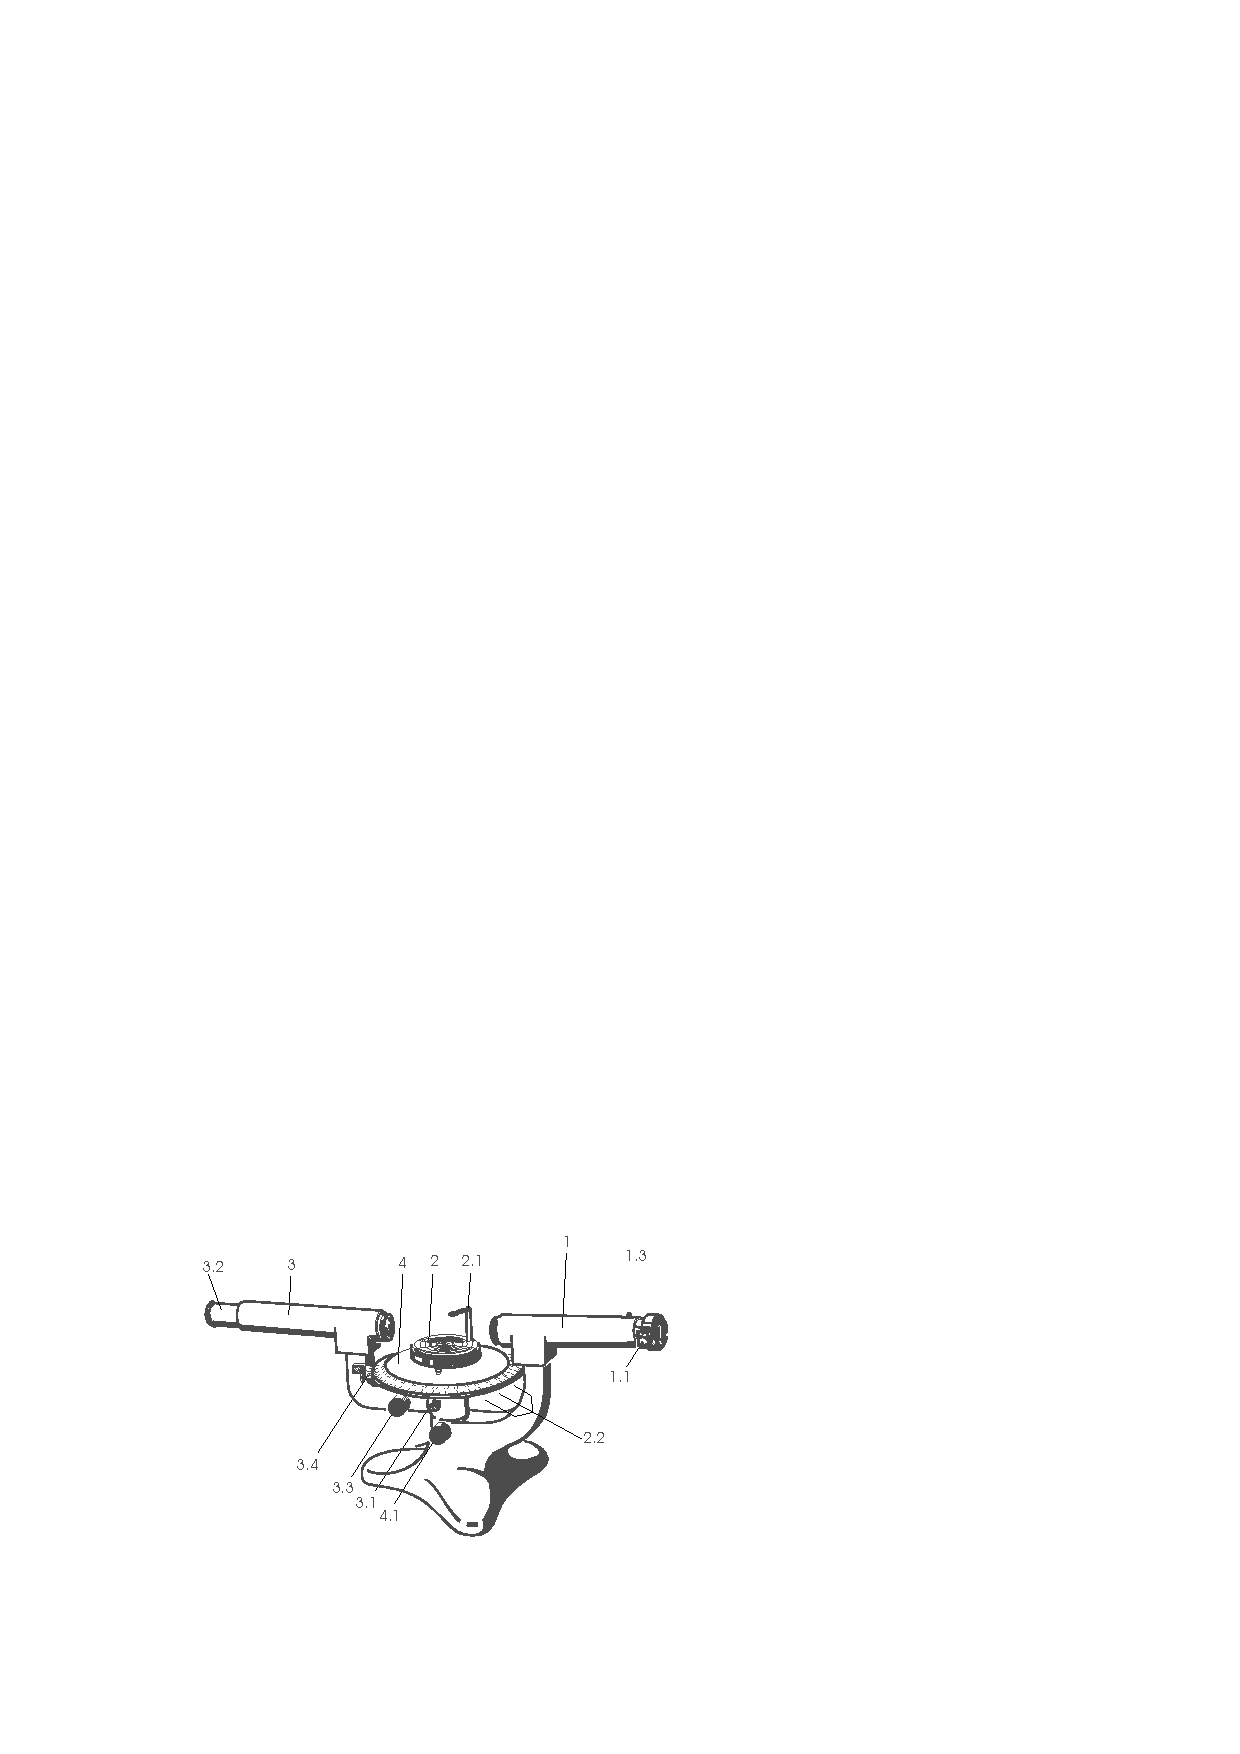
\includegraphics[scale=0.8]{content/aufbau1.pdf}
\caption{Gitterspektralapparat\cite{anleitung605}.}
  \label{fig:spektralap}
\end{figure}
Abbildung \ref{fig:spektralap} zeigt den Aufbau des verwendeten Gitterspektralapparates. Dieser besteht aus einem Kollimatorrohr 1 mit Spaltblende 1.1, einem Gittertisch 2, einem schwenkbarem Fernrohr 3 und einer Teilkreisplatte 4. Die Lichtquelle wird vor dem Spalt 1.1 positioniert. Die Strahlen werden durch eine Objektivlinse gebündelt, treffen auf das Gitter, wo diese gebeugt werden. Durch das Fernrohr, welches aus einer Objektiv- und einer Okularlinse mit Fadenkreuz besteht, kann man die vom Gitter gebeugten Strahlen beobachten. Das Fernrohr wird so bewegt, dass die gewünschten Spektrallinien zu sehen sind. Der entsprechende Winkel wird an der Teilkreisplatte abgelesen.

\subsection{Beugungswinkel für Helium, Natrium, Kalium und Rubidium}
Zunächst werden mit dem Gitterspektralapparat die Beugungswinkel der Spektrallinien von Helium gemessen. Dazu wird die Helium-lampe vor den Spalt gestellt. Das Fernrohr wird zunächst so eingestellt, dass die dunkelrote Linie des Spektrums sichtbar ist. Der dazugehörige Winkel wird an der Teilkreisplatte abgelesen und notiert. Dies wird für alle weiteren Linien des Spektrums wiederholt.
Anschließend sollen die Mittelwerte der Dubletts von Natrium, Kalium und Rubidium ausgemessen werden. Bei Natrium wird ein rotes, ein gelbes und ein grünes Dublett ausgemesse und bei Kalium zwei gelbe und zwei grüne Dubletts. Bei Rubidium wird das Dublett zwischen der dritten und der vierten Linie gemessen.

\subsection{Eichung des Okularmiktometers}
Zur Eichung des Okularmikrometers werden die grünen und violetten Spektrallinien verwendet. Der Abstand der Spektrallinien wird mit einem Okularmikrometer ausgemessen. Dazu wird das Fadenkreuz mit dem Drehknopf mit 100 eingravierten Strichen an der Seite des Fernrohrs verschoben. Die erhaltene Differenz der Wellenlängen der Dublettlinien liegt zunächst in Einheiten der telung des Okularmikrometers vor. Die tatsächliche Wellenlänge berechnet sich mit der Gleichung
\begin{equation}
   \Delta \lambda = \frac{\cos\overline{\phi}}{\cos\overline{\phi_1,2}}\frac{\Delta s}{\Delta t}(\lambda_1 -\lambda_2)
 \end{equation}
